\chapter{Single-Photon Emission Computed Tomography (SPECT)}
\label{ch:spect}

% Chapter-opening illustrated modality infographic.
\begin{center}
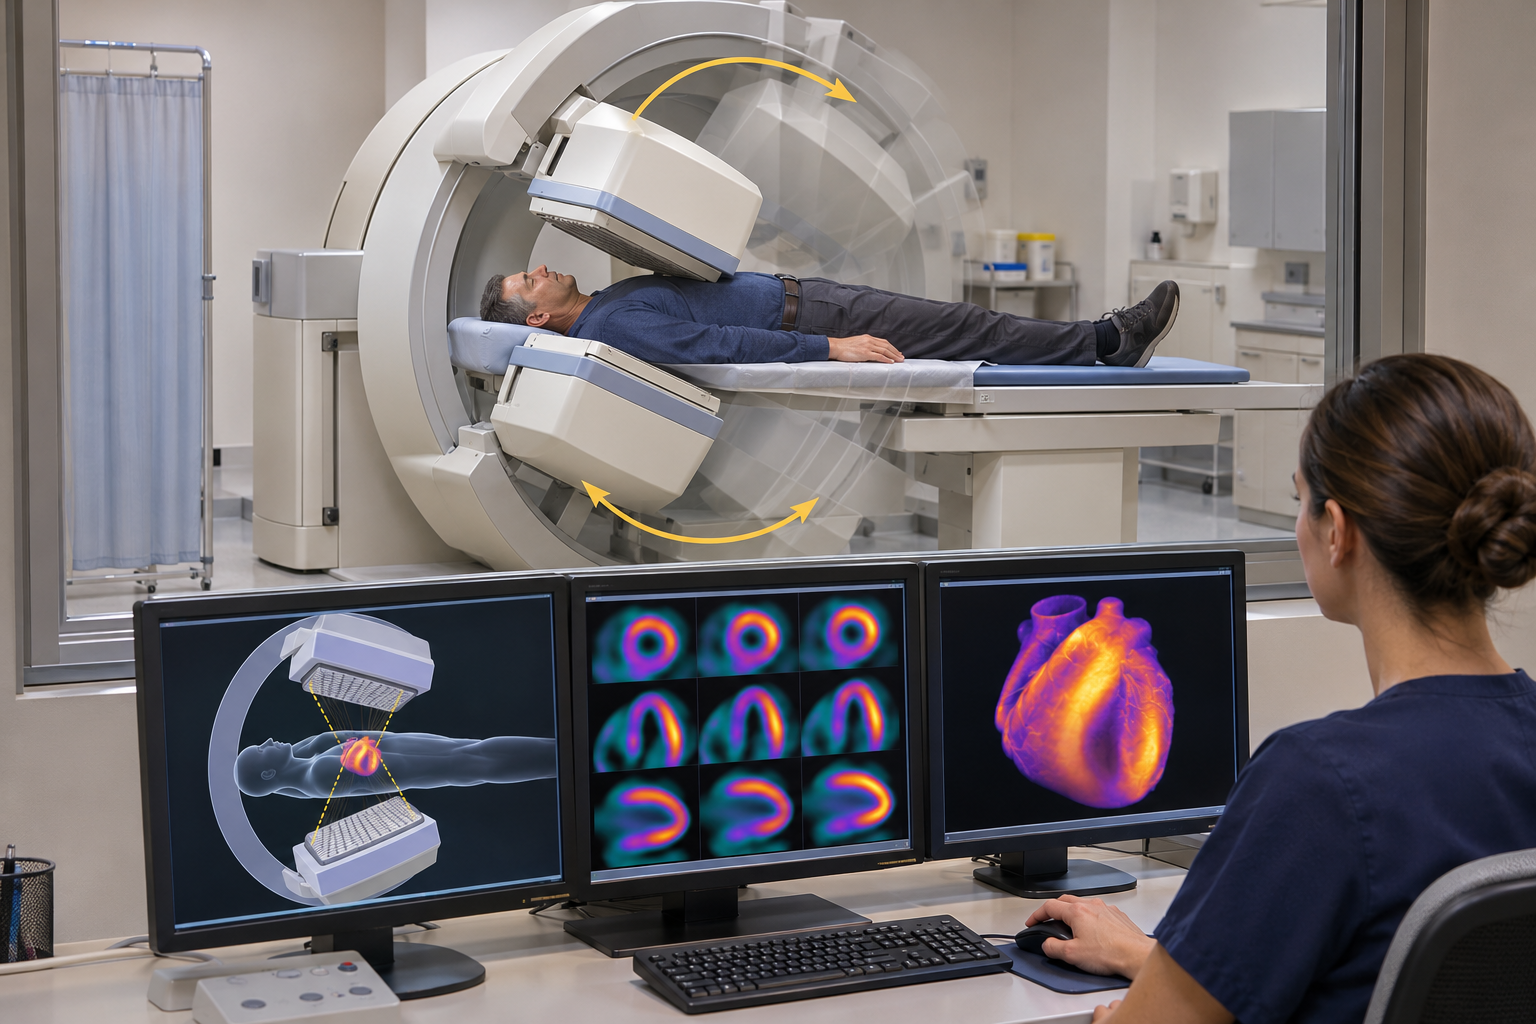
\includegraphics[width=\textwidth,keepaspectratio]{modalities/infographics/spect_realistic.png}
\end{center}
\begin{center}\footnotesize SPECT camera heads rotate around the patient and reconstruct detected single gamma photons into a three-dimensional tracer distribution. AI-generated illustration; perfusion images are not clinical studies.\end{center}

\section{Overview}
Single-Photon Emission Computed Tomography (SPECT) is a nuclear medicine imaging technique that uses gamma cameras to detect photons emitted by radiopharmaceuticals administered to a patient. Computational reconstruction generates three-dimensional images of radiotracer distribution within the body.

Unlike CT and structural MRI, SPECT primarily provides information about physiological function, tissue perfusion, metabolic processes, molecular transport, and receptor availability. It is particularly valuable for myocardial perfusion imaging, skeletal disorders, neurological diseases, parathyroid localization, and infection imaging.

This catalogue focuses specifically on SPECT and SPECT/CT, excluding PET and examinations predominantly performed using planar scintigraphy. 

Some listed examinations are usually performed with planar imaging; they are included only where SPECT or SPECT/CT can provide selected three-dimensional localization, which is identified in the relevant entries.

\section{Where SPECT is used}
The numbered entries summarize characteristic SPECT findings and radiopharmaceuticals. Interpretation should account for the tracer's biological mechanism, acquisition protocol, physiological state, and reconstruction method.

\subsection{Cardiovascular diseases}
\begin{enumerate}[leftmargin=*,itemsep=0.45em,topsep=0.4em]
\item \textbf{Cardiac device infection.} Useful imaging findings include: Abnormal leukocyte uptake around implanted devices. Radiopharmaceutical: ⁹⁹ᵐTc-HMPAO leukocytes.
\item \textbf{Cardiac sympathetic denervation.} Useful imaging findings include: Reduced myocardial sympathetic tracer uptake. Radiopharmaceutical: ¹²³I-MIBG.
\item \textbf{Chronic heart failure.} Useful imaging findings include: Reduced ventricular function and possible perfusion abnormalities. Radiopharmaceutical: ⁹⁹ᵐTc-Sestamibi.
\item \textbf{Coronary artery disease.} Useful imaging findings include: Stress-induced myocardial perfusion defects. Radiopharmaceutical: ⁹⁹ᵐTc-Sestamibi.
\item \textbf{Coronary microvascular dysfunction.} Useful imaging findings include: Reduced myocardial flow reserve on specialized dynamic SPECT. Radiopharmaceutical: ⁹⁹ᵐTc-Sestamibi.
\item \textbf{Dilated cardiomyopathy.} Useful imaging findings include: Ventricular dilatation and reduced ejection fraction. Radiopharmaceutical: ⁹⁹ᵐTc-Sestamibi.
\item \textbf{Hibernating myocardium.} Useful imaging findings include: Preserved or redistributing tracer uptake in dysfunctional myocardium. Radiopharmaceutical: ²⁰¹Tl-Chloride.
\item \textbf{Hypertrophic cardiomyopathy.} Useful imaging findings include: Heterogeneous myocardial perfusion. Radiopharmaceutical: ⁹⁹ᵐTc-Tetrofosmin.
\item \textbf{Ischemic cardiomyopathy.} Useful imaging findings include: Regional perfusion defects and ventricular dysfunction. Radiopharmaceutical: ⁹⁹ᵐTc-Sestamibi.
\item \textbf{Left ventricular aneurysm.} Useful imaging findings include: Fixed perfusion defect and dyskinetic ventricular segment. Radiopharmaceutical: ⁹⁹ᵐTc-Sestamibi.
\item \textbf{Multivessel coronary artery disease.} Useful imaging findings include: Perfusion abnormalities involving multiple vascular territories. Radiopharmaceutical: ⁹⁹ᵐTc-Tetrofosmin.
\item \textbf{Myocardial ischemia.} Useful imaging findings include: Reversible myocardial perfusion defects. Radiopharmaceutical: ⁹⁹ᵐTc-Tetrofosmin.
\item \textbf{Previous myocardial infarction.} Useful imaging findings include: Fixed myocardial perfusion defects. Radiopharmaceutical: ⁹⁹ᵐTc-Sestamibi.
\item \textbf{Prosthetic valve endocarditis.} Useful imaging findings include: Abnormal periprosthetic leukocyte accumulation. Radiopharmaceutical: ⁹⁹ᵐTc-HMPAO leukocytes.
\item \textbf{Transthyretin cardiac amyloidosis.} Useful imaging findings include: Myocardial uptake confirmed on SPECT and interpreted with validated criteria. Radiopharmaceutical: ⁹⁹ᵐTc-PYP, DPD, HMDP.
\end{enumerate}
Myocardial perfusion imaging is one of the most established and widely used clinical applications of SPECT. Balanced ischemia in multivessel coronary disease can, however, produce apparently normal relative perfusion images.
For bone-tracer assessment of ATTR cardiac amyloidosis, evaluate for a monoclonal protein and interpret uptake with the clinical findings; uptake alone does not establish ATTR and can be misleading in AL amyloidosis.

\subsection{Neurological and neurodegenerative diseases}
\begin{enumerate}[leftmargin=*,itemsep=0.45em,topsep=0.4em]
\item \textbf{Alzheimer disease.} Useful imaging findings include: Temporoparietal and posterior cingulate hypoperfusion. Radiopharmaceutical: ⁹⁹ᵐTc-HMPAO.
\item \textbf{Cerebral circulatory arrest.} Useful imaging findings include: Absence of intracranial radiotracer perfusion on a protocol-based ancillary study. Radiopharmaceutical: ⁹⁹ᵐTc-HMPAO.
\item \textbf{Corticobasal syndrome.} Useful imaging findings include: Asymmetric cortical perfusion abnormalities or reduced dopamine transporter binding. Radiopharmaceutical: ⁹⁹ᵐTc-ECD, ¹²³I-Ioflupane.
\item \textbf{Dementia with Lewy bodies.} Useful imaging findings include: Reduced striatal dopamine transporter binding. Radiopharmaceutical: ¹²³I-Ioflupane.
\item \textbf{Drug-induced parkinsonism.} Useful imaging findings include: Usually preserved dopamine transporter binding in pure drug-induced cases. Radiopharmaceutical: ¹²³I-Ioflupane.
\item \textbf{Essential tremor.} Useful imaging findings include: Usually preserved striatal dopamine transporter binding. Radiopharmaceutical: ¹²³I-Ioflupane.
\item \textbf{Frontotemporal dementia.} Useful imaging findings include: Frontal and anterior temporal hypoperfusion. Radiopharmaceutical: ⁹⁹ᵐTc-ECD.
\item \textbf{Huntington disease.} Useful imaging findings include: Reported basal ganglia perfusion abnormalities. Radiopharmaceutical: ⁹⁹ᵐTc-HMPAO.
\item \textbf{Hypoxic-ischemic brain injury.} Useful imaging findings include: Regional or widespread perfusion reduction. Radiopharmaceutical: ⁹⁹ᵐTc-ECD.
\item \textbf{Multiple system atrophy.} Useful imaging findings include: Reduced striatal dopamine transporter binding. Radiopharmaceutical: ¹²³I-Ioflupane.
\item \textbf{Normal pressure hydrocephalus.} Useful imaging findings include: Variable cerebral perfusion abnormalities. Radiopharmaceutical: ⁹⁹ᵐTc-ECD.
\item \textbf{Parkinson disease.} Useful imaging findings include: Reduced striatal dopamine transporter binding. Radiopharmaceutical: ¹²³I-Ioflupane.
\item \textbf{Progressive supranuclear palsy.} Useful imaging findings include: Reduced striatal dopamine transporter binding. Radiopharmaceutical: ¹²³I-Ioflupane.
\item \textbf{Vascular dementia.} Useful imaging findings include: Multifocal cerebral perfusion abnormalities. Radiopharmaceutical: ⁹⁹ᵐTc-HMPAO.
\end{enumerate}
Dopamine transporter SPECT (DaT-SPECT) can help distinguish degenerative parkinsonian syndromes from certain nondegenerative causes of tremor. It cannot reliably distinguish Parkinson disease from multiple system atrophy or progressive supranuclear palsy.
Radionuclide cerebral perfusion imaging may serve as an ancillary test in death by neurologic criteria when performed and interpreted under applicable protocols; the scan alone does not establish that clinical diagnosis.

\subsection{Epilepsy}
\begin{enumerate}[leftmargin=*,itemsep=0.45em,topsep=0.4em]
\item \textbf{Drug-resistant focal epilepsy.} Useful imaging findings include: Regional ictal hyperperfusion associated with seizure onset or propagation. Radiopharmaceutical: ⁹⁹ᵐTc-HMPAO.
\item \textbf{Focal cortical dysplasia.} Useful imaging findings include: Abnormal ictal regional perfusion. Radiopharmaceutical: ⁹⁹ᵐTc-HMPAO.
\item \textbf{Frontal lobe epilepsy.} Useful imaging findings include: Ictal frontal hyperperfusion. Radiopharmaceutical: ⁹⁹ᵐTc-ECD.
\item \textbf{Mesial temporal sclerosis.} Useful imaging findings include: Variable interictal temporal hypoperfusion. Radiopharmaceutical: ⁹⁹ᵐTc-ECD.
\item \textbf{MRI-negative focal epilepsy.} Useful imaging findings include: Potential localization of seizure-related perfusion abnormalities. Radiopharmaceutical: ⁹⁹ᵐTc-HMPAO.
\item \textbf{Occipital lobe epilepsy.} Useful imaging findings include: Ictal occipital hyperperfusion. Radiopharmaceutical: ⁹⁹ᵐTc-HMPAO.
\item \textbf{Parietal lobe epilepsy.} Useful imaging findings include: Ictal parietal hyperperfusion. Radiopharmaceutical: ⁹⁹ᵐTc-ECD.
\item \textbf{Temporal lobe epilepsy.} Useful imaging findings include: Ictal temporal hyperperfusion. Radiopharmaceutical: ⁹⁹ᵐTc-HMPAO.
\end{enumerate}
A specialized computational technique called SISCOM (Subtraction Ictal SPECT Co-registered to MRI) compares ictal and interictal SPECT studies to help localize epileptogenic regions before surgery.

\subsection{Cerebrovascular diseases}
\begin{enumerate}[leftmargin=*,itemsep=0.45em,topsep=0.4em]
\item \textbf{Carotid artery occlusion.} Useful imaging findings include: Regional hypoperfusion. Radiopharmaceutical: ⁹⁹ᵐTc-ECD.
\item \textbf{Carotid artery stenosis.} Useful imaging findings include: Reduced cerebrovascular perfusion reserve. Radiopharmaceutical: ⁹⁹ᵐTc-HMPAO.
\item \textbf{Cerebral hyperperfusion syndrome.} Useful imaging findings include: Increased regional perfusion following revascularization. Radiopharmaceutical: ⁹⁹ᵐTc-ECD.
\item \textbf{Cerebral small vessel disease.} Useful imaging findings include: Heterogeneous cerebral perfusion. Radiopharmaceutical: ⁹⁹ᵐTc-HMPAO.
\item \textbf{Cerebral vasospasm.} Useful imaging findings include: Regional perfusion reduction. Radiopharmaceutical: ⁹⁹ᵐTc-ECD.
\item \textbf{Chronic cerebral ischemia.} Useful imaging findings include: Persistently reduced regional perfusion. Radiopharmaceutical: ⁹⁹ᵐTc-ECD.
\item \textbf{Ischemic stroke.} Useful imaging findings include: Regional cerebral hypoperfusion. Radiopharmaceutical: ⁹⁹ᵐTc-HMPAO.
\item \textbf{Moyamoya disease.} Useful imaging findings include: Impaired cerebral perfusion and vascular reserve. Radiopharmaceutical: ⁹⁹ᵐTc-HMPAO.
\end{enumerate}
Most acute cerebrovascular diseases are now investigated primarily using CT, CT angiography, or MRI. SPECT remains useful in selected cerebral perfusion and vascular reserve assessments.

\subsection{Pulmonary diseases}
\begin{enumerate}[leftmargin=*,itemsep=0.45em,topsep=0.4em]
\item \textbf{Acute pulmonary embolism.} Useful imaging findings include: Segmental ventilation-perfusion mismatch. Radiopharmaceutical: ⁹⁹ᵐTc-MAA and Technegas.
\item \textbf{Chronic obstructive pulmonary disease.} Useful imaging findings include: Heterogeneous ventilation and perfusion. Radiopharmaceutical: ⁹⁹ᵐTc-MAA and Technegas.
\item \textbf{Chronic pulmonary embolism.} Useful imaging findings include: Persistent regional perfusion defects; ventilation imaging helps determine whether defects are mismatched. Radiopharmaceutical: ⁹⁹ᵐTc-MAA; add a ventilation agent when performing V/Q imaging.
\item \textbf{Chronic thromboembolic pulmonary hypertension.} Useful imaging findings include: Persistent mismatched ventilation-perfusion defects. Radiopharmaceutical: ⁹⁹ᵐTc-MAA and a ventilation agent (e.g., ⁹⁹ᵐTc-Technegas or aerosol).
\item \textbf{Pneumonia.} Useful imaging findings include: Ventilation and perfusion abnormalities, sometimes with reverse mismatch. Radiopharmaceutical: ⁹⁹ᵐTc-MAA and Technegas.
\item \textbf{Pulmonary artery obstruction.} Useful imaging findings include: Regional absence of pulmonary perfusion. Radiopharmaceutical: ⁹⁹ᵐTc-MAA.
\item \textbf{Pulmonary artery stenosis.} Useful imaging findings include: Reduced perfusion within the affected lung region. Radiopharmaceutical: ⁹⁹ᵐTc-MAA.
\item \textbf{Pulmonary emphysema.} Useful imaging findings include: Regional reductions in ventilation and perfusion. Radiopharmaceutical: ⁹⁹ᵐTc-MAA and Technegas.
\item \textbf{Pulmonary fibrosis (selected preoperative regional function assessment).} Useful imaging findings include: Regional perfusion contribution to lung function; does not diagnose pulmonary fibrosis. Radiopharmaceutical: ⁹⁹ᵐTc-MAA.
\end{enumerate}

\subsection{Thyroid and parathyroid diseases}
\begin{enumerate}[leftmargin=*,itemsep=0.45em,topsep=0.4em]
\item \textbf{Ectopic parathyroid adenoma.} Useful imaging findings include: Focal uptake outside the expected parathyroid location. Radiopharmaceutical: ⁹⁹ᵐTc-Sestamibi.
\item \textbf{Ectopic thyroid tissue.} Useful imaging findings include: Uptake at an abnormal anatomical location; SPECT/CT may aid localization. Radiopharmaceutical: ⁹⁹ᵐTc-Pertechnetate.
\item \textbf{Follicular thyroid carcinoma.} Useful imaging findings include: Radioiodine-avid metastases; SPECT/CT is a localization adjunct. Radiopharmaceutical: ¹³¹I.
\item \textbf{Papillary thyroid carcinoma.} Useful imaging findings include: Radioiodine-avid residual or metastatic tissue; SPECT/CT adds localization to planar imaging. Radiopharmaceutical: ¹³¹I.
\item \textbf{Parathyroid adenoma.} Useful imaging findings include: Persistent focal radiotracer retention. Radiopharmaceutical: ⁹⁹ᵐTc-Sestamibi.
\item \textbf{Parathyroid carcinoma.} Useful imaging findings include: Possible increased focal tracer uptake. Radiopharmaceutical: ⁹⁹ᵐTc-Sestamibi.
\item \textbf{Parathyroid hyperplasia.} Useful imaging findings include: Abnormal uptake involving one or more glands. Radiopharmaceutical: ⁹⁹ᵐTc-Sestamibi.
\item \textbf{Recurrent hyperparathyroidism.} Useful imaging findings include: Focal uptake corresponding to residual or recurrent hyperfunctioning tissue. Radiopharmaceutical: ⁹⁹ᵐTc-Sestamibi.
\item \textbf{Retrosternal goiter.} Useful imaging findings include: Thyroid tracer uptake extending into the mediastinum. Radiopharmaceutical: ¹²³I.
\item \textbf{Thyroid cancer bone metastases.} Useful imaging findings include: Focal skeletal radioiodine uptake; SPECT/CT may localize selected lesions. Radiopharmaceutical: ¹³¹I.
\item \textbf{Thyroid cancer lymph node metastases.} Useful imaging findings include: Focal radioiodine uptake; SPECT/CT may anatomically localize selected lesions. Radiopharmaceutical: ¹³¹I.
\item \textbf{Thyroid cancer pulmonary metastases.} Useful imaging findings include: Focal or diffuse pulmonary radioiodine uptake, generally assessed on planar imaging. Radiopharmaceutical: ¹³¹I.
\end{enumerate}
Routine thyroid function scintigraphy is generally performed using planar imaging. SPECT/CT is particularly helpful when precise anatomical localization is required.
Radioiodine whole-body imaging for thyroid cancer is commonly acquired as planar imaging; SPECT/CT is an adjunct for anatomical localization or characterization of selected findings.

\subsection{Bone and skeletal diseases}
\begin{enumerate}[leftmargin=*,itemsep=0.45em,topsep=0.4em]
\item \textbf{Acute osteomyelitis.} Useful imaging findings include: Increased uptake in infected skeletal structures. Radiopharmaceutical: ⁹⁹ᵐTc-MDP.
\item \textbf{Breast cancer bone metastases.} Useful imaging findings include: Focal or multifocal increased skeletal uptake. Radiopharmaceutical: ⁹⁹ᵐTc-MDP.
\item \textbf{Chronic osteomyelitis.} Useful imaging findings include: Abnormal osseous uptake or leukocyte accumulation. Radiopharmaceutical: Labeled leukocytes.
\item \textbf{Delayed fracture union.} Useful imaging findings include: Variable abnormal uptake at fracture site. Radiopharmaceutical: ⁹⁹ᵐTc-MDP.
\item \textbf{Ewing sarcoma.} Useful imaging findings include: Variable increased skeletal uptake. Radiopharmaceutical: ⁹⁹ᵐTc-MDP.
\item \textbf{Femoral neck stress fracture.} Useful imaging findings include: Focal increased femoral neck uptake. Radiopharmaceutical: ⁹⁹ᵐTc-MDP.
\item \textbf{Fibrous dysplasia.} Useful imaging findings include: Increased skeletal remodeling activity. Radiopharmaceutical: ⁹⁹ᵐTc-MDP.
\item \textbf{Fracture nonunion.} Useful imaging findings include: Abnormal uptake reflecting residual biological activity. Radiopharmaceutical: ⁹⁹ᵐTc-MDP.
\item \textbf{Heterotopic ossification.} Useful imaging findings include: Increased extraosseous tracer accumulation. Radiopharmaceutical: ⁹⁹ᵐTc-MDP.
\item \textbf{Hypertrophic osteoarthropathy.} Useful imaging findings include: Symmetrical periosteal uptake. Radiopharmaceutical: ⁹⁹ᵐTc-MDP.
\item \textbf{Insufficiency fracture.} Useful imaging findings include: Increased uptake within mechanically weakened bone. Radiopharmaceutical: ⁹⁹ᵐTc-MDP.
\item \textbf{Medial tibial stress syndrome.} Useful imaging findings include: Longitudinal increased tibial uptake. Radiopharmaceutical: ⁹⁹ᵐTc-MDP.
\item \textbf{Occult fracture.} Useful imaging findings include: Focal skeletal tracer accumulation. Radiopharmaceutical: ⁹⁹ᵐTc-MDP.
\item \textbf{Osteoblastic bone metastases.} Useful imaging findings include: Multifocal increased skeletal uptake. Radiopharmaceutical: ⁹⁹ᵐTc-MDP.
\item \textbf{Osteoblastoma.} Useful imaging findings include: Increased uptake within affected bone. Radiopharmaceutical: ⁹⁹ᵐTc-MDP.
\item \textbf{Osteochondral lesion of the talus.} Useful imaging findings include: Focal subchondral tracer accumulation. Radiopharmaceutical: ⁹⁹ᵐTc-MDP.
\item \textbf{Osteoid osteoma.} Useful imaging findings include: Intense focal tracer uptake. Radiopharmaceutical: ⁹⁹ᵐTc-MDP.
\item \textbf{Osteonecrosis.} Useful imaging findings include: Reduced uptake in necrotic regions or increased reparative uptake. Radiopharmaceutical: ⁹⁹ᵐTc-MDP.
\item \textbf{Osteosarcoma.} Useful imaging findings include: Increased uptake in mineralizing tumor components. Radiopharmaceutical: ⁹⁹ᵐTc-MDP.
\item \textbf{Paget disease of bone.} Useful imaging findings include: Intense uptake involving affected bone. Radiopharmaceutical: ⁹⁹ᵐTc-MDP.
\item \textbf{Prostate cancer bone metastases.} Useful imaging findings include: Increased osteoblastic activity. Radiopharmaceutical: ⁹⁹ᵐTc-MDP.
\item \textbf{Sacral insufficiency fracture.} Useful imaging findings include: Characteristic sacral uptake, sometimes H-shaped. Radiopharmaceutical: ⁹⁹ᵐTc-MDP.
\item \textbf{Stress fracture.} Useful imaging findings include: Focal or linear increased bone uptake. Radiopharmaceutical: ⁹⁹ᵐTc-MDP.
\item \textbf{Vertebral compression fracture.} Useful imaging findings include: Increased uptake in active or healing fractures. Radiopharmaceutical: ⁹⁹ᵐTc-MDP.
\end{enumerate}

\subsection{Joint and prosthetic disorders}
\begin{enumerate}[leftmargin=*,itemsep=0.45em,topsep=0.4em]
\item \textbf{Aseptic prosthetic loosening.} Useful imaging findings include: Increased uptake at prosthetic interfaces. Radiopharmaceutical: ⁹⁹ᵐTc-MDP.
\item \textbf{Charcot arthropathy.} Useful imaging findings include: Increased joint and skeletal remodeling activity. Radiopharmaceutical: ⁹⁹ᵐTc-MDP.
\item \textbf{Complex regional pain syndrome.} Useful imaging findings include: Variable periarticular uptake abnormalities. Radiopharmaceutical: ⁹⁹ᵐTc-MDP.
\item \textbf{Mandibular condylar hyperplasia.} Useful imaging findings include: Asymmetric increased condylar uptake. Radiopharmaceutical: ⁹⁹ᵐTc-MDP.
\item \textbf{Osteoarthritis.} Useful imaging findings include: Increased subchondral bone turnover. Radiopharmaceutical: ⁹⁹ᵐTc-MDP.
\item \textbf{Painful total hip arthroplasty.} Useful imaging findings include: Abnormal acetabular or femoral component uptake. Radiopharmaceutical: ⁹⁹ᵐTc-MDP.
\item \textbf{Painful total knee arthroplasty.} Useful imaging findings include: Abnormal compartmental or periprosthetic uptake. Radiopharmaceutical: ⁹⁹ᵐTc-MDP.
\item \textbf{Patellofemoral osteoarthritis.} Useful imaging findings include: Increased patellofemoral tracer uptake. Radiopharmaceutical: ⁹⁹ᵐTc-MDP.
\item \textbf{Prosthetic joint infection.} Useful imaging findings include: Abnormal periprosthetic leukocyte accumulation; interpretation may require complementary bone or marrow imaging. Radiopharmaceutical: ¹¹¹In-oxine leukocytes, with bone or marrow imaging as indicated.
\item \textbf{Rheumatoid arthritis.} Useful imaging findings include: Increased periarticular skeletal uptake. Radiopharmaceutical: ⁹⁹ᵐTc-MDP.
\item \textbf{Sacroiliac joint dysfunction.} Useful imaging findings include: Variable increased sacroiliac uptake. Radiopharmaceutical: ⁹⁹ᵐTc-MDP.
\item \textbf{Sacroiliitis.} Useful imaging findings include: Increased sacroiliac bone turnover in some cases. Radiopharmaceutical: ⁹⁹ᵐTc-MDP.
\item \textbf{Septic arthritis.} Useful imaging findings include: Increased inflammatory tracer accumulation. Radiopharmaceutical: Labeled leukocytes.
\item \textbf{Temporomandibular joint degeneration.} Useful imaging findings include: Increased condylar uptake. Radiopharmaceutical: ⁹⁹ᵐTc-MDP.
\end{enumerate}

\subsection{Spine disorders}
\begin{enumerate}[leftmargin=*,itemsep=0.45em,topsep=0.4em]
\item \textbf{Baastrup disease.} Useful imaging findings include: Increased uptake between adjacent spinous processes. Radiopharmaceutical: ⁹⁹ᵐTc-MDP.
\item \textbf{Cervical facet arthropathy.} Useful imaging findings include: Focal increased facet joint uptake. Radiopharmaceutical: ⁹⁹ᵐTc-MDP.
\item \textbf{Degenerative disc disease.} Useful imaging findings include: Increased uptake at adjacent vertebral endplates. Radiopharmaceutical: ⁹⁹ᵐTc-MDP.
\item \textbf{Lumbar facet arthropathy.} Useful imaging findings include: Increased facet joint uptake. Radiopharmaceutical: ⁹⁹ᵐTc-MDP.
\item \textbf{Spinal fusion pseudarthrosis.} Useful imaging findings include: Persistent focal uptake at fusion site. Radiopharmaceutical: ⁹⁹ᵐTc-MDP.
\item \textbf{Spinal hardware loosening.} Useful imaging findings include: Increased uptake around orthopedic instrumentation. Radiopharmaceutical: ⁹⁹ᵐTc-MDP.
\item \textbf{Spinal metastases.} Useful imaging findings include: Focal abnormal vertebral uptake. Radiopharmaceutical: ⁹⁹ᵐTc-MDP.
\item \textbf{Spondylodiscitis.} Useful imaging findings include: Increased uptake involving adjacent vertebral endplates. Radiopharmaceutical: ⁶⁷Ga-Citrate, ⁹⁹ᵐTc-MDP.
\item \textbf{Spondylolisthesis.} Useful imaging findings include: Abnormal uptake in mechanically stressed structures. Radiopharmaceutical: ⁹⁹ᵐTc-MDP.
\item \textbf{Spondylolysis.} Useful imaging findings include: Increased uptake within an active pars interarticularis lesion. Radiopharmaceutical: ⁹⁹ᵐTc-MDP.
\item \textbf{Vertebral osteomyelitis.} Useful imaging findings include: Abnormal vertebral skeletal or inflammatory uptake. Radiopharmaceutical: ⁹⁹ᵐTc-MDP.
\end{enumerate}

\subsection{Infectious and inflammatory diseases}
\begin{enumerate}[leftmargin=*,itemsep=0.45em,topsep=0.4em]
\item \textbf{Crohn disease.} Useful imaging findings include: Segmental inflammatory bowel uptake. Radiopharmaceutical: ⁹⁹ᵐTc-HMPAO leukocytes.
\item \textbf{Diabetic foot osteomyelitis.} Useful imaging findings include: Abnormal leukocyte accumulation within bone. Radiopharmaceutical: ⁹⁹ᵐTc-HMPAO leukocytes.
\item \textbf{Diabetic foot soft-tissue infection.} Useful imaging findings include: Leukocyte uptake confined to soft tissues. Radiopharmaceutical: ⁹⁹ᵐTc-HMPAO leukocytes.
\item \textbf{Fever of unknown origin.} Useful imaging findings include: Potential localization of occult inflammatory or infectious foci. Radiopharmaceutical: ⁶⁷Ga-Citrate.
\item \textbf{Infected orthopedic hardware.} Useful imaging findings include: Abnormal peri-implant leukocyte accumulation; correlate with bone or marrow imaging when indicated. Radiopharmaceutical: ¹¹¹In-oxine leukocytes, with bone or marrow imaging as indicated.
\item \textbf{Inflammatory bowel disease.} Useful imaging findings include: Increased bowel leukocyte accumulation. Radiopharmaceutical: ⁹⁹ᵐTc-HMPAO leukocytes.
\item \textbf{Intra-abdominal abscess.} Useful imaging findings include: Focal leukocyte accumulation. Radiopharmaceutical: ¹¹¹In-Oxine leukocytes.
\item \textbf{Occult infection.} Useful imaging findings include: Abnormal localized inflammatory tracer uptake. Radiopharmaceutical: Labeled leukocytes.
\item \textbf{Pulmonary tuberculosis.} Useful imaging findings include: Abnormal inflammatory tracer accumulation. Radiopharmaceutical: ⁶⁷Ga-Citrate.
\item \textbf{Sarcoidosis.} Useful imaging findings include: Increased inflammatory tracer uptake. Radiopharmaceutical: ⁶⁷Ga-Citrate.
\item \textbf{Ulcerative colitis.} Useful imaging findings include: Increased colonic leukocyte accumulation. Radiopharmaceutical: ⁹⁹ᵐTc-HMPAO leukocytes.
\item \textbf{Vascular graft infection.} Useful imaging findings include: Abnormal leukocyte uptake surrounding vascular graft. Radiopharmaceutical: ⁹⁹ᵐTc-HMPAO leukocytes.
\end{enumerate}
Several gallium-67 and labeled leukocyte examinations have been superseded by FDG-PET/CT or other modalities in many clinical settings.

\subsection{Neuroendocrine and adrenal tumors}
\begin{enumerate}[leftmargin=*,itemsep=0.45em,topsep=0.4em]
\item \textbf{Aldosterone-producing adrenal adenoma.} Useful imaging findings include: Asymmetric adrenal cortical tracer uptake. Radiopharmaceutical: ¹³¹I-NP-59.
\item \textbf{Autonomous adrenal cortisol production.} Useful imaging findings include: Asymmetric adrenal cortical tracer uptake. Radiopharmaceutical: ¹³¹I-NP-59.
\item \textbf{Bronchial carcinoid.} Useful imaging findings include: Increased somatostatin receptor uptake. Radiopharmaceutical: ¹¹¹In-Pentetreotide.
\item \textbf{Gastrinoma.} Useful imaging findings include: Abnormal receptor-specific uptake. Radiopharmaceutical: ¹¹¹In-Pentetreotide.
\item \textbf{Gastroenteropancreatic neuroendocrine tumor.} Useful imaging findings include: Increased somatostatin receptor tracer uptake. Radiopharmaceutical: ¹¹¹In-Pentetreotide.
\item \textbf{Metastatic neuroblastoma.} Useful imaging findings include: Multifocal MIBG-avid lesions. Radiopharmaceutical: ¹²³I-MIBG.
\item \textbf{Metastatic pheochromocytoma.} Useful imaging findings include: Abnormal MIBG uptake in metastatic lesions. Radiopharmaceutical: ¹²³I-MIBG.
\item \textbf{Neuroblastoma.} Useful imaging findings include: Increased catecholamine transporter-related uptake. Radiopharmaceutical: ¹²³I-MIBG.
\item \textbf{Pancreatic neuroendocrine tumor.} Useful imaging findings include: Focal receptor-specific tracer accumulation. Radiopharmaceutical: ¹¹¹In-Pentetreotide.
\item \textbf{Paraganglioma.} Useful imaging findings include: Focal extra-adrenal MIBG accumulation. Radiopharmaceutical: ¹²³I-MIBG.
\item \textbf{Pheochromocytoma.} Useful imaging findings include: Abnormal adrenal MIBG accumulation. Radiopharmaceutical: ¹²³I-MIBG.
\item \textbf{Small bowel neuroendocrine tumor.} Useful imaging findings include: Increased receptor-specific uptake. Radiopharmaceutical: ¹¹¹In-Pentetreotide.
\end{enumerate}
Somatostatin receptor PET/CT has largely replaced conventional indium-111 receptor scintigraphy where available. Adrenal cortical scintigraphy with NP-59 is now uncommon.

\subsection{Renal and urinary diseases}
\begin{enumerate}[leftmargin=*,itemsep=0.45em,topsep=0.4em]
\item \textbf{Acute pyelonephritis.} Useful imaging findings include: Focal renal cortical uptake defects. Radiopharmaceutical: ⁹⁹ᵐTc-DMSA.
\item \textbf{Duplex kidney.} Useful imaging findings include: Abnormal renal cortical configuration. Radiopharmaceutical: ⁹⁹ᵐTc-DMSA.
\item \textbf{Ectopic kidney.} Useful imaging findings include: Functioning renal tissue at an abnormal anatomical location. Radiopharmaceutical: ⁹⁹ᵐTc-DMSA.
\item \textbf{Horseshoe kidney.} Useful imaging findings include: Abnormal three-dimensional renal configuration. Radiopharmaceutical: ⁹⁹ᵐTc-DMSA.
\item \textbf{Reflux nephropathy.} Useful imaging findings include: Abnormal cortical tracer distribution. Radiopharmaceutical: ⁹⁹ᵐTc-DMSA.
\item \textbf{Renal cortical scarring.} Useful imaging findings include: Persistent cortical tracer defects. Radiopharmaceutical: ⁹⁹ᵐTc-DMSA.
\item \textbf{Renal dysplasia.} Useful imaging findings include: Reduced or heterogeneous cortical uptake. Radiopharmaceutical: ⁹⁹ᵐTc-DMSA.
\item \textbf{Renal infarction.} Useful imaging findings include: Regional absence of cortical uptake. Radiopharmaceutical: ⁹⁹ᵐTc-DMSA.
\end{enumerate}
SPECT provides supplementary three-dimensional renal cortical information. Dynamic renal functional studies are predominantly performed using conventional gamma-camera renography.

\subsection{Hepatobiliary, gastrointestinal and splenic diseases}
\begin{enumerate}[leftmargin=*,itemsep=0.45em,topsep=0.4em]
\item \textbf{Accessory spleen (selected SPECT/CT localization).} Useful imaging findings include: Focal uptake corresponding to functioning splenic tissue; planar imaging is also used. Radiopharmaceutical: ⁹⁹ᵐTc-Heat-damaged RBCs.
\item \textbf{Active gastrointestinal bleeding (selected SPECT localization).} Useful imaging findings include: Extravascular blood-pool accumulation; planar imaging is generally performed first. Radiopharmaceutical: ⁹⁹ᵐTc-labeled RBCs.
\item \textbf{Bile leak (selected SPECT/CT localization).} Useful imaging findings include: Extraluminal biliary tracer; planar hepatobiliary imaging is generally the initial study. Radiopharmaceutical: ⁹⁹ᵐTc-Mebrofenin.
\item \textbf{Focal nodular hyperplasia (selected SPECT/CT characterization).} Useful imaging findings include: Preserved or increased colloid uptake in some lesions; planar imaging is commonly used. Radiopharmaceutical: ⁹⁹ᵐTc-Sulfur colloid.
\item \textbf{Functional splenic tissue within an abdominal mass (selected SPECT/CT localization).} Useful imaging findings include: Selective splenic tracer accumulation; planar imaging is also used. Radiopharmaceutical: ⁹⁹ᵐTc-Heat-damaged RBCs.
\item \textbf{Hepatic hemangioma (selected SPECT/CT localization).} Useful imaging findings include: Delayed blood-pool tracer accumulation; planar blood-pool imaging is commonly used first. Radiopharmaceutical: ⁹⁹ᵐTc-labeled RBCs.
\item \textbf{Intrahepatic hepatopulmonary shunting before radioembolization.} Useful imaging findings include: Planar imaging quantifies pulmonary shunting; SPECT/CT may provide selected localization. Radiopharmaceutical: ⁹⁹ᵐTc-MAA.
\item \textbf{Meckel diverticulum (selected SPECT/CT localization).} Useful imaging findings include: Ectopic gastric mucosal tracer uptake; SPECT/CT may clarify equivocal planar findings. Radiopharmaceutical: ⁹⁹ᵐTc-Pertechnetate.
\item \textbf{Splenosis (selected SPECT/CT localization).} Useful imaging findings include: Tracer uptake within ectopic splenic tissue; planar imaging is also used. Radiopharmaceutical: ⁹⁹ᵐTc-Heat-damaged RBCs.
\end{enumerate}

\subsection{Lymphatic disorders and oncological localization}
\begin{enumerate}[leftmargin=*,itemsep=0.45em,topsep=0.4em]
\item \textbf{Breast carcinoma sentinel node localization.} Useful imaging findings include: Identification of draining sentinel lymph nodes. Radiopharmaceutical: ⁹⁹ᵐTc-Nanocolloid.
\item \textbf{Chylous leakage.} Useful imaging findings include: Abnormal lymphatic tracer accumulation. Radiopharmaceutical: ⁹⁹ᵐTc-Nanocolloid.
\item \textbf{Lymphatic obstruction.} Useful imaging findings include: Interrupted or delayed lymphatic drainage. Radiopharmaceutical: ⁹⁹ᵐTc-Nanocolloid.
\item \textbf{Malignant melanoma sentinel node localization.} Useful imaging findings include: Identification of regional draining lymph nodes. Radiopharmaceutical: ⁹⁹ᵐTc-Nanocolloid.
\item \textbf{Oral carcinoma sentinel node localization.} Useful imaging findings include: Localization of cervical sentinel nodes. Radiopharmaceutical: ⁹⁹ᵐTc-Nanocolloid.
\item \textbf{Penile carcinoma sentinel node localization.} Useful imaging findings include: Localization of inguinal sentinel nodes. Radiopharmaceutical: ⁹⁹ᵐTc-Nanocolloid.
\item \textbf{Primary lymphedema.} Useful imaging findings include: Abnormal lymphatic drainage and dermal backflow. Radiopharmaceutical: ⁹⁹ᵐTc-Nanocolloid.
\item \textbf{Secondary lymphedema.} Useful imaging findings include: Impaired lymphatic transport. Radiopharmaceutical: ⁹⁹ᵐTc-Nanocolloid.
\end{enumerate}
Lymphoscintigraphy and sentinel-node mapping commonly use planar imaging; SPECT/CT is a selected adjunct when planar localization is inadequate or anatomically complex. Sentinel-node imaging identifies drainage pathways and does not establish whether nodes contain malignant cells.

\subsection{Breast diseases}
Dedicated molecular breast imaging generally uses planar gamma-camera systems. The entries below refer only to specialized or limited dedicated breast SPECT applications and are not routine indications for conventional SPECT.
\begin{enumerate}[leftmargin=*,itemsep=0.45em,topsep=0.4em]
\item \textbf{Invasive ductal carcinoma.} Useful imaging findings include: Focal increased radiotracer accumulation. Radiopharmaceutical: ⁹⁹ᵐTc-Sestamibi.
\item \textbf{Invasive lobular carcinoma.} Useful imaging findings include: Variable increased tracer uptake. Radiopharmaceutical: ⁹⁹ᵐTc-Sestamibi.
\item \textbf{Multifocal breast carcinoma.} Useful imaging findings include: Multiple regions of abnormal tracer accumulation. Radiopharmaceutical: ⁹⁹ᵐTc-Sestamibi.
\item \textbf{Recurrent breast carcinoma.} Useful imaging findings include: Abnormal focal tracer uptake. Radiopharmaceutical: ⁹⁹ᵐTc-Sestamibi.
\end{enumerate}
These are specialized or limited applications rather than standard indications for conventional SPECT.

\subsection{Summary of catalogue}
\begin{center}
\begin{tabular}{@{}p{0.70\textwidth}r@{}}
\toprule
\textbf{Disease category} & \textbf{Entries} \\
\midrule
Bone and skeletal diseases & 24 \\
Breast diseases & 4 \\
Cardiovascular diseases & 15 \\
Cerebrovascular diseases & 8 \\
Epilepsy & 8 \\
Hepatobiliary, gastrointestinal and splenic diseases & 9 \\
Infectious and inflammatory diseases & 12 \\
Joint and prosthetic disorders & 14 \\
Lymphatic disorders and oncological localization & 8 \\
Neuroendocrine and adrenal tumors & 12 \\
Neurological and neurodegenerative diseases & 14 \\
Pulmonary diseases & 9 \\
Renal and urinary diseases & 8 \\
Spine disorders & 11 \\
Thyroid and parathyroid diseases & 12 \\
\midrule
\textbf{Total} & \textbf{168} \\
\bottomrule
\end{tabular}
\end{center}

\subsection{Types of SPECT imaging}
\begin{longtable}{@{}p{0.38\textwidth}p{0.54\textwidth}@{}}
\toprule
\textbf{Technique} & \textbf{Primary application} \\
\midrule
\endfirsthead
\toprule
\textbf{Technique} & \textbf{Primary application} \\
\midrule
\endhead
Bone SPECT/CT & Skeletal remodeling and lesion localization \\
Cerebral perfusion SPECT & Regional cerebral blood flow assessment \\
Conventional SPECT & Three-dimensional radiotracer distribution \\
CZT-SPECT & High-sensitivity semiconductor detector imaging \\
Dopamine transporter SPECT & Degenerative parkinsonian syndromes \\
Dynamic SPECT & Time-dependent radiotracer distribution \\
Gated SPECT & Cardiac motion and ventricular function \\
Ictal SPECT & Seizure localization \\
Interictal SPECT & Baseline cerebral perfusion \\
Leukocyte SPECT/CT & Infection localization \\
Pinhole SPECT & High-resolution imaging of small structures \\
Quantitative SPECT & Absolute or relative radiotracer concentration \\
Somatostatin receptor SPECT & Neuroendocrine tumor imaging \\
SPECT/CT & Combined functional and anatomical imaging \\
Stress-rest myocardial SPECT & Myocardial ischemia and infarction \\
Ventilation-perfusion SPECT & Pulmonary embolism \\
\bottomrule
\end{longtable}

\subsection{Major SPECT radiopharmaceuticals}
\begin{longtable}{@{}p{0.30\textwidth}p{0.40\textwidth}p{0.22\textwidth}@{}}
\toprule
\textbf{Radiopharmaceutical} & \textbf{Biological process or target} & \textbf{Photon energy} \\
\midrule
\endfirsthead
\toprule
\textbf{Radiopharmaceutical} & \textbf{Biological process or target} & \textbf{Photon energy} \\
\midrule
\endhead
²⁰¹Tl-Chloride & Perfusion and myocardial viability & Approximately 68--80 keV, additional emissions \\
¹²³I-Ioflupane & Dopamine transporters & 159 keV \\
¹²³I-MIBG & Norepinephrine transport & 159 keV \\
¹³¹I-Sodium iodide & Thyroid iodine transport & 364 keV \\
¹¹¹In-Oxine leukocytes & Leukocyte migration & 171, 245 keV \\
¹¹¹In-Pentetreotide & Somatostatin receptors & 171, 245 keV \\
⁶⁷Ga-Citrate & Inflammatory and tumor-associated accumulation & 93, 185, 300 keV \\
⁹⁹ᵐTc-DMSA & Renal cortical retention & 140 keV \\
⁹⁹ᵐTc-DPD & Bone-seeking tracer retention & 140 keV \\
⁹⁹ᵐTc-ECD & Cerebral perfusion & 140 keV \\
⁹⁹ᵐTc-HDP & Bone remodeling & 140 keV \\
⁹⁹ᵐTc-HMDP & Bone-seeking tracer retention & 140 keV \\
⁹⁹ᵐTc-HMPAO & Cerebral perfusion & 140 keV \\
⁹⁹ᵐTc-HMPAO leukocytes & Leukocyte migration & 140 keV \\
⁹⁹ᵐTc-MAA & Pulmonary perfusion & 140 keV \\
⁹⁹ᵐTc-MDP & Bone remodeling & 140 keV \\
⁹⁹ᵐTc-Mebrofenin & Hepatobiliary transport & 140 keV \\
⁹⁹ᵐTc-Nanocolloid & Lymphatic transport & 140 keV \\
⁹⁹ᵐTc-PYP & Bone-seeking tracer retention & 140 keV \\
⁹⁹ᵐTc-Sestamibi & Tissue perfusion and mitochondrial retention & 140 keV \\
⁹⁹ᵐTc-Tetrofosmin & Myocardial perfusion & 140 keV \\
\bottomrule
\end{longtable}

\subsection{Physical principles of SPECT}
Radioactive decay of the administered radiopharmaceutical produces gamma photons detected by a rotating gamma-camera system. The decay process is described by:
\begin{equation}
A(t)=A_0 e^{-\lambda t},
\end{equation}
where $A(t)$ is the activity at time $t$, $A_0$ is the initial activity, $\lambda$ is the decay constant, and $t$ is elapsed time. The relationship between half-life and decay constant is:
\begin{equation}
T_{1/2}=\frac{\ln 2}{\lambda}.
\end{equation}
Measured SPECT projection data can be represented with the simplified imaging model:
\begin{equation}
\mathbf{y}\sim\operatorname{Poisson}(\mathbf{H}\mathbf{x}+\mathbf{r}),
\end{equation}
where $\mathbf{y}$ represents measured photon counts, $\mathbf{x}$ the unknown three-dimensional activity distribution, $\mathbf{H}$ the imaging system response, and $\mathbf{r}$ background and scattered photon contributions.

\subsection{Reconstruction algorithms}
\begin{longtable}{@{}p{0.48\textwidth}p{0.44\textwidth}@{}}
\toprule
\textbf{Algorithm} & \textbf{Application} \\
\midrule
\endfirsthead
\toprule
\textbf{Algorithm} & \textbf{Application} \\
\midrule
\endhead
Deep learning reconstruction & Emerging noise reduction and reconstruction techniques \\
Filtered back projection (FBP) & Conventional analytical reconstruction \\
MAP reconstruction & Regularized statistical reconstruction \\
Maximum likelihood expectation maximization (MLEM) & Statistical iterative reconstruction \\
Ordered subsets expectation maximization (OSEM) & Accelerated iterative reconstruction \\
Resolution recovery reconstruction & Compensation for detector and collimator limitations \\
\bottomrule
\end{longtable}

\subsection{Quantitative SPECT parameters}
\begin{longtable}{@{}p{0.34\textwidth}p{0.16\textwidth}p{0.42\textwidth}@{}}
\toprule
\textbf{Parameter} & \textbf{Abbreviation} & \textbf{Clinical significance} \\
\midrule
\endfirsthead
\toprule
\textbf{Parameter} & \textbf{Abbreviation} & \textbf{Clinical significance} \\
\midrule
\endhead
Activity concentration & --- & Radioactive activity per unit tissue volume \\
Differential renal uptake & DRU & Relative functioning renal cortical tissue \\
End-diastolic volume & EDV & Ventricular filling volume \\
End-systolic volume & ESV & Residual ventricular volume after contraction \\
Heart-to-contralateral lung ratio & H/CL & Supplementary cardiac amyloidosis assessment \\
Heart-to-mediastinum ratio & H/M & Cardiac sympathetic innervation \\
Left ventricular ejection fraction & LVEF & Ventricular systolic function \\
Myocardial blood flow & MBF & Quantitative myocardial perfusion \\
Myocardial flow reserve & MFR & Stress-to-rest blood flow ratio \\
Regional cerebral blood flow & rCBF & Regional cerebral perfusion \\
Specific binding ratio & SBR & Striatal dopamine transporter binding \\
Standardized uptake value & SUV & Normalized quantitative tracer uptake \\
Summed difference score & SDS & Reversible myocardial perfusion abnormalities \\
Summed rest score & SRS & Myocardial perfusion abnormalities at rest \\
Summed stress score & SSS & Myocardial perfusion abnormalities during stress \\
Target-to-background ratio & TBR & Relative lesion tracer accumulation \\
Total perfusion deficit & TPD & Extent and severity of myocardial perfusion defects \\
Transient ischemic dilatation ratio & TID & Marker associated with extensive myocardial ischemia \\
\bottomrule
\end{longtable}

\subsection{SPECT versus PET}
\begin{longtable}{@{}p{0.29\textwidth}p{0.31\textwidth}p{0.31\textwidth}@{}}
\toprule
\textbf{Feature} & \textbf{SPECT} & \textbf{PET} \\
\midrule
\endfirsthead
\toprule
\textbf{Feature} & \textbf{SPECT} & \textbf{PET} \\
\midrule
\endhead
Bone imaging & Widely established & Available with selected tracers \\
Cardiac perfusion imaging & Widely established & Established \\
Collimation & Physical collimation & Electronic coincidence localization \\
Common radionuclides & ⁹⁹ᵐTc, ¹²³I, ¹¹¹In & ¹⁸F, ⁶⁸Ga, ¹¹C, ⁸²Rb \\
Detection mechanism & Individual gamma photons & Coincident annihilation photons \\
Detection sensitivity & Generally lower & Generally higher \\
Equipment cost & Generally lower & Generally higher \\
Full name & Single-photon emission computed tomography & Positron emission tomography \\
Hybrid imaging & SPECT/CT & PET/CT, PET/MRI \\
Oncological imaging & Selected applications & Extensive applications \\
Photon energy & Radionuclide-dependent & 511 keV \\
Quantitative accuracy & More technically challenging & Generally superior \\
Radiopharmaceutical availability & Often more widely available & More dependent on production and distribution infrastructure \\
Typical clinical spatial resolution & Approximately 7--15 mm & Approximately 4--6 mm \\
\bottomrule
\end{longtable}
Spatial resolution depends on detector technology, collimator design, reconstruction methods, and acquisition protocols.

\subsection{Established clinical applications versus research applications}
\begin{longtable}{@{}p{0.54\textwidth}p{0.40\textwidth}@{}}
\toprule
\textbf{Application} & \textbf{Clinical status} \\
\midrule
\endfirsthead
\toprule
\textbf{Application} & \textbf{Clinical status} \\
\midrule
\endhead
Bone metastasis detection & Established \\
Cerebral perfusion reserve assessment & Specialized clinical application \\
Degenerative parkinsonian syndrome assessment & Established \\
Myocardial ischemia assessment & Established \\
Myocardial perfusion imaging & Established \\
Neuroblastoma imaging & Established \\
Parathyroid adenoma localization & Established \\
Presurgical epilepsy localization & Specialized clinical application \\
Prosthetic joint infection assessment & Established in selected cases \\
Psychiatric disorder diagnosis & Investigational and not clinically validated \\
Pulmonary embolism detection & Established \\
Quantitative myocardial blood flow & Emerging and technology-dependent \\
Quantitative skeletal disease assessment & Emerging \\
Radioiodine-avid thyroid cancer localization & Established \\
Sentinel lymph node localization & Established \\
Skeletal pain localization & Established in selected cases \\
Transthyretin cardiac amyloidosis assessment & Established with appropriate diagnostic criteria \\
Traumatic brain injury classification & Investigational \\
\bottomrule
\end{longtable}

\subsection{Published SPECT imaging datasets and resources}
\begin{longtable}{@{}p{0.40\textwidth}p{0.52\textwidth}@{}}
\toprule
\textbf{Source} & \textbf{Primary utility} \\
\midrule
\endfirsthead
\toprule
\textbf{Source} & \textbf{Primary utility} \\
\midrule
\endhead
American Society of Nuclear Cardiology & Myocardial perfusion imaging \\
European Association of Nuclear Medicine & Clinical protocols and imaging standards \\
International Atomic Energy Agency & Nuclear medicine technical resources \\
OpenGATE & Monte Carlo simulations of nuclear medicine imaging \\
Parkinson's Progression Markers Initiative (PPMI) & Dopamine transporter SPECT \\
PubMed Central & Published clinical SPECT images \\
Radiopaedia & Annotated clinical SPECT cases \\
Society of Nuclear Medicine and Molecular Imaging & Clinical imaging guidelines \\
STIR & Open-source tomographic reconstruction software \\
The Cancer Imaging Archive & Selected nuclear medicine imaging datasets \\
\bottomrule
\end{longtable}

\subsection{Recommended metadata for a SPECT imaging dataset}
\begin{longtable}{@{}p{0.45\textwidth}p{0.49\textwidth}@{}}
\toprule
\textbf{Attribute} & \textbf{Example} \\
\midrule
Acquisition matrix & $128 \times 128$ \\
Acquisition protocol & Stress-rest \\
Administered activity & 370 MBq \\
Attenuation correction & CT-based \\
Cardiac gating & 8 frames per cardiac cycle \\
Collimator & Low-energy high-resolution \\
Detector type & NaI(Tl) scintillation detector \\
Diagnostic reference standard & Independently established clinical diagnosis \\
Disease & Coronary artery disease \\
Image format & DICOM \\
Image license & CC BY or other specified license \\
Imaging modality & Gated SPECT/CT \\
Number of projections & 64 \\
Photon energy & 140 keV \\
Physical half-life & Approximately 6 hours \\
Publication reference & DOI or PMID \\
Radiological finding & Reversible inferior myocardial perfusion defect \\
Radionuclide & Technetium-99m \\
Radiopharmaceutical & ⁹⁹ᵐTc-Sestamibi \\
Reconstruction algorithm & OSEM \\
Resolution recovery & Applied \\
Scatter correction & Applied \\
Summed difference score & 8 \\
Summed rest score & 4 \\
Summed stress score & 12 \\
Uptake period & 60 minutes \\
\bottomrule
\end{longtable}

\subsection{Image dimensionality and tracer interpretation}
SPECT should be treated as a quantitative, radiopharmaceutical-dependent, three-dimensional functional imaging modality.
\begin{center}
\begin{tabular}{@{}ll@{}}
\toprule
\textbf{Imaging modality} & \textbf{Data dimensionality} \\
\midrule
CT & $X, Y, Z$ \\
Diffusion MRI & $X, Y, Z$, diffusion encoding \\
Dynamic SPECT & $X, Y, Z$, time \\
fMRI & $X, Y, Z$, time \\
Gated SPECT & $X, Y, Z$, physiological phase \\
Planar scintigraphy & $X, Y$ \\
SPECT/CT & Co-registered functional and anatomical volumes \\
Static SPECT & $X, Y, Z$ \\
Structural MRI & $X, Y, Z$ per sequence \\
X-ray & $X, Y$ \\
\bottomrule
\end{tabular}
\end{center}

For AI-based diagnostic systems, increased or decreased tracer uptake must be interpreted in the context of its biological mechanism.
\begin{longtable}{@{}p{0.35\textwidth}p{0.59\textwidth}@{}}
\toprule
\textbf{Radiopharmaceutical} & \textbf{Increased uptake may indicate} \\
\midrule
\endfirsthead
\toprule
\textbf{Radiopharmaceutical} & \textbf{Increased uptake may indicate} \\
\midrule
\endhead
Labeled leukocytes & Accumulation of inflammatory cells \\
¹²³I-Ioflupane & Preserved dopamine transporter availability \\
¹²³I-MIBG & Preserved norepinephrine transport or neuroendocrine tumor uptake \\
¹³¹I-Sodium iodide & Functioning iodine-avid thyroid tissue \\
⁹⁹ᵐTc-HMPAO & Increased regional cerebral perfusion \\
⁹⁹ᵐTc-MDP & Increased skeletal remodeling \\
⁹⁹ᵐTc-Sestamibi & Preserved myocardial perfusion or mitochondrial retention \\
\bottomrule
\end{longtable}

The radiopharmaceutical, acquisition protocol, physiological state, and reconstruction parameters should be mandatory inputs to a comprehensive SPECT diagnostic model. 

